\chapter{Spoken Dialogue Systems}
\label{chap:spoken_dialogue_systems}

\lettrine{T}{his} chapter gives an overview on \aclp{sds}, including common architectures, different system types, and implementation techniques.
The concept of adaptive \aclp{sds}, which is a core topic in this work, is introduced as well, along with the challenges involved and examples of possible adaptation strategies on different levels.
%The parallelisms to the human perspective are highlighted along the way to help to understand the motivations and goals.

\pagebreak

\acresetall

\noindent
\Acfp{sds} offer a wide range of services and are used on daily basis in various forms, both for commercial and personal purposes.
The main difference between them and other ways to communicate with computers is the use of speech -- and mostly speech alone -- for interaction.
This offers benefits to the users, like being able to perform tasks while keeping their hands free, contrary to systems that require textual input from a keyboard or haptic touch on a screen.
We are witnessing an ever-growing presence of voice-activated devices, like speech-activated cars, hands-free medical assistants, and \acp{its}.
These devices support more and more functionalities in a way that is more comfortable and intuitive for users.
It can be expected that in the near future such devices will be used not only by individuals but also in more social contexts, including interactions where multiple humans are involved.
This makes the understanding and improvement of social skills in \acp{sds} all the more important.

The common architecture of \acp{sds} is explained in \cref{sec:architecture_sds}, along with details about each component and how it can be implemented.
\Cref{sec:types_of_sdss} gives an overview of applications that use a \ac{sds} at their core to communicate with users.
A roadmap toward \acp{sds} with vocal accommodation capabilities as well as the challenges involved in that are discussed in \cref{sec:adaptive_spoken_dialogue_systems}.
Ultimately, such capabilities would improve the personalization and overall experience of the interaction.

\section{Architecture of \aclp{sds}}
\label{sec:architecture_sds}

As shown in \cref{fig:sds_architecture}, the architecture of a \ac{sds} is symmetric in terms of input and output types.
Each cycle starts and ends with speech signals, generated first by the user, and then by the system (more sophisticated systems can also take the initiative).
The content of the utterance, usually referred to as \emph{intent}, is then extracted to determine the utterance's objective.
Similarly, the system's speech output is based on generated content that captures some intent.
The \enquote{brain} at the core of the cycle decides what intent is most suitable for the user's input.
This can be done purely by learning from provided dialogue examples, using the help of external information or databases, based on hand-crafted rules, or some combination of those.
This simplified flow assumes that the user and the system take turns alternately, one at a time.
However, one interlocutor may of course need multiple consecutive turns to convey the message due to length or no response from the other interlocutor.
Although each component is a whole research area by itself, there are numerous open-source implementations that help to quickly build a basic fully functioning system and focus on a specific one.
Brief overviews of these \ac{nlp} tasks are given in \crefrange{subsec:automatic_speech_recognition}{subsec:text-to-speech_synthesis}.
Note that this is a basic typical architecture and each component may be extended or modified.
Specifically, this architecture changes substantially in fully neural-based systems.
However, even in that case, the general flow (and by extension the training data) remains the same.
%
\begin{figure}[t]
	\centering
	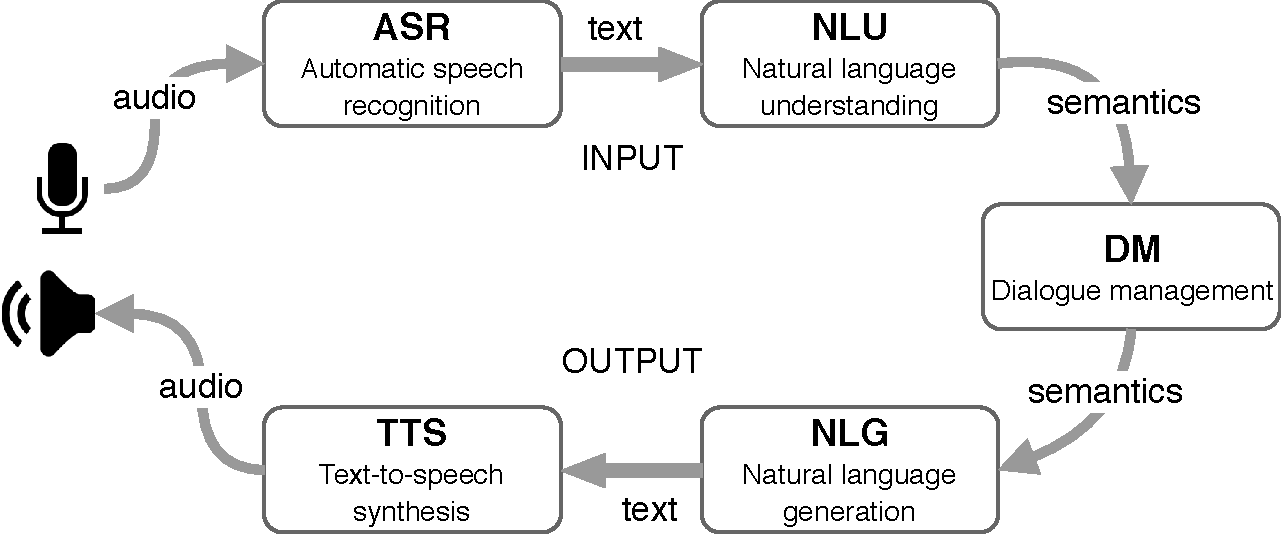
\includegraphics[width=\linewidth]{sds_architecture}
	\caption[Architecture of a spoken dialogue system]
	{A typical architecture of a spoken dialogue system.
	The interaction lifecycle is symmetric, and for each analysis input step there is a corresponding generation output step.
	The exchange usually starts with a user spoken utterance and ends with the system's spoken response.}
	\label{fig:sds_architecture}
\end{figure}

\subsection{\Acl{asr}}
\label{subsec:automatic_speech_recognition}

An essential condition for verbal communication is to be able to hear what the interlocutor says and process it into words.
For computer, this is done using \acf{asr}, which translates the audio signals produced by the user's articulators into a machine-readable form that can subsequently be fed to the \ac{nlu} component.
This step is crucial for vocal accommodation, as it is the only component that accesses the audio signal.
However, \acp{sds} predominantly merely use it to extract the said words and discard it afterwards.
As a result, they know \emph{what} was said by the user but not \emph{how} it was said.
For any kind of responsive behavior, this component must be extended to provide some additional information about the input speech.

\subsubsection{Tools}
\label{subsubsec:tools_asr}

Kaldi \citep{Povey2011kaldi} and CMU Sphinx \citep{Lamere2003sphinx} are free-to-use \ac{asr} engines that offer various functionalities, including training a model on a custom dataset.
For the purpose of vocal accommodation, one benefit of using such modifiable toolkits is the ability to access the phoneme times.
This is crucial for detecting and tracking certain phonetic features, and segmental ones in particular (as in \cref{chap:convergence_module_for_sdss}).

\subsection{\Acl{nlu}}
\label{subsec:natural_language_understanding}

After getting the words uttered by the user, the system needs to infer an intention from them, i.e., what the user wanted to achieve in that turn.
This is the role of the \acf{nlu} component.
An intention can be as simple as asking the \ac{sds} to perform a task (e.g., to turn on the radio in a voice-activated car).
such requests are mostly recognizable by pre-defined keywords the system can look for in the transcribed input text.
Other requests, like inquiring information about a place or booking a flight, require the system to be able to withdraw -- and properly formulate -- information from some source.
Such tasks require further information (e.g., flight origin and destination, date, price range, etc.) to be obtained, or, if that information is not provided by the user, additional turns where the system asks for the missing bits.
This process is called slot-filling.
More complex reactions, and especially in the case of chatbots, demands deeper semantic analysis, as the intention might not be explicitly articulated and in some cases, such a defined intention may not even exist.

%\subsubsection{Tools}
%\label{subsubsec:tools_nlu}

\subsection{\Acl{dm}}
\label{subsec:dialogue_management}

After completing processing the user's input, a decision must be made by the \ac{sds} as to how to react.
This is done by the \acf{dm}, which is the central component of a \ac{sds}.
The \ac{dm} is typically divided into \emph{belief tracker} and \emph{policy} modules.
The former accumulates information regarding the user's wish based on current and previous turns, while the latter is responsible for determining the most appropriate response to that intention.
If any additional data is required for satisfying the user's needs, e.g., some information from the web or a database, the retrieval will be done by the \ac{dm}.
The same goes for specific domain knowledge, which can be made available to the system.
Deciding on the best action can be achieved using a deterministic rule system for a small number of simple cases (a \ac{cnc} system, for example), but need more sophisticated models for more involved situations.
One commonly used technique is reinforcement learning, which is suitable for making selecting an action based on a given state.
All these conditions determine how flexible and elaborate the system is, and specifically what domain(s) it can handle.

%\subsubsection{Tools}
%\label{subsubsec:tools_dm}

\subsection{\Acl{nlg}}
\label{subsec:natural_language_generation}

After deciding on the most appropriate response to the user, the system needs to convey it in a human-understandable manner, namely words.
The process is reversed to \ac{nlu}, i.e., generating text based on a given intent.
Depending on the user's input intent, the system may respond with simple acknowledgment statements, repetition and information approval, or completely newly formed full sentences.
Additional challenges of this task often root from things that could be reduced or ignored in \ac{nlu}, but must be precise in \ac{nlg}.
For example, using wrong verb conjugations and tenses will cause the system's response to sound ungrammatical or ill-formed in some cases, but could even lead to a misunderstanding of the system's response.
Therefore, depending on the language, the \ac{nlg} component should be aware of the user's gender, the number of users speaking to it, the nature of the user's intent and how it may be carried out, and more (in multimodal systems, these may influence other modalities as well).

%\subsubsection{Tools}
%\label{subsubsec:tools_nlg}

\subsection{\Acl{tts} synthesis}
\label{subsec:text-to-speech_synthesis}

The last step in the flow is converting the text provided by the \ac{nlg} component to speech signal and play it to the user.
This is performed using a \acf{tts} module, which takes orthographic forms of words and outputs a voice that utters them.
Traditionally, voices are learned from recorded human speech by selecting and concatenating small units of it.
Linguistic analyses are performed to translate the orthographic forms to sound sequences, insert stresses and pauses, etc.
Additional properties, like the contour and duration, are usually determined in inference time.
Newer methods are mostly neural-based and can generate audio frames directly from text \citep[e.g.,][]{Shen2018natural}.
All these methods have the limitation of not being able to control the generation process directly in each utterance, especially not on the segmental level.
This makes it hard to apply detected changes in the user's speech, which is a major barrier on the way to integrate accommodation capabilities into \acp{sds}.
Nevertheless, there are examples of \acp{sds} that can adapt on various levels, including specific modifications in speech (see \cref{sec:adaptive_spoken_dialogue_systems}).

\subsubsection{Tools}
\label{subsubsec:tools_tts}

Free \ac{tts} engines for training voices include Festival \citep{Black1997festival}, espeak \citep{Duddington2012espeak}, and MaryTTS \citep{Schroder2011open}.
In addition to being used as complete \ac{tts} pipelines, these systems can also provide intermediate analysis outputs like phonetic transcriptions.

\section{Types of \aclp{sds}}
\label{sec:types_of_sdss}

By and large, \acp{sds} can be divided into two main categories, which determine the communication style and behavior of the system: task-oriented systems \citep[e.g.,][]{Wen2016network, Zhao2016towards} and chatbots systems \citep[e.g.,][]{Vinyals2015neural, Li2016deep}.
The former has a well-defined scope and aims to achieve a specific goal, while the latter is open-ended with no specific task in mind other than sustaining the conversation with the user.
\Cref{tab:sds_types} compares these two system types.
Vocal accommodation is relevant for both these system categories, but in different ways.
Task-oriented systems may need to accommodate faster and introduce changes more frequently.
It might also be required to reset the system's speech for each interaction if it's used by more than one user or for different purposes.
Chatbots, on the other hand, might be able to exploit the fact that they are usually involved in longer conversations, giving them more time to learn the user's vocal behavior.
This could lead to a slower, smoother process, which should gradually improve the personalization of the system.
Another category is voice-activated \acf{cnc} systems, which are arguably not \acp{sds} per se, since they only rarely engage in conversation or trigger a multi-turn dialogue.
Therefore, such systems leave little room for accommodation to occur.
Nevertheless, \ac{cnc} systems are considered a simple kind of task-oriented \ac{sds} in this work, as ultimately they are designed to achieve a specific task, even if a dialogue is not necessarily required for that.
Indeed, task-oriented systems like \acp{pa} often offer \ac{cnc} interfaces as well.
\Acp{sds} can be utilized in various ways and be embedded in different types of systems.
\Crefrange{subsec:personal_assistants}{subsec:virtual_humans} survey some of the main system types with a \ac{sds} at their core.
%
\begin{table}[tb]
	\centering
	\caption[Types of \aclp{sds}: Task-oriented vs.\ Chatbots]{A comparison of some characteristics in task-oriented \acp{sds} and chatbots.}
	\label{tab:sds_types}
	\begin{tabularx}{\linewidth}{>{\bfseries}lp{.38\linewidth}p{.37\linewidth}}
		\toprule
		\vspace{.3cm}
							& \multicolumn{1}{c}{{\large \textbf{Task-oriented}}} & \multicolumn{1}{c}{{\large \textbf{Chatbots}}} \\
		\vspace{.2cm}
		Goal				& Help the user achieve a specific, pre-defined goal
							& Converse as naturally and continuously as possible \\
		\vspace{.2cm}
		Applications		& \Aclp{pa}, \ac{cnc} systems, in-car voice-activated systems, reservations, etc.
							& Free-form \acl{c-ai} applications: chitchat bots, social robots, etc. \\
		\vspace{.2cm}
		Domain				& Domain-specific and/or multi-domain
							& Domain-free or robust cross-domain \\
		\vspace{.2cm}
		Modeling			& Statistical models and/or handcrafted rules
							& Typically \ac{s2s} models with no-go filters \\
		\vspace{.2cm}
		Evaluation			& Task completion rate and completion time, number of turns (+ subjective criteria)
							& Chat length, relevant replies ratio, user engagement, general user satisfaction \\
		\bottomrule
	\end{tabularx}
\end{table}
%
\subsection{\Aclp{pa}}
\label{subsec:personal_assistants}

A \acl{pa} (\acs{pa}; also \emph{intelligent \acl{pa}} or \emph{virtual \acl{pa}}\footnote{The term \emph{virtual assistant} is widely used as well.
However, it is avoided here, since it also refers to a different kind of occupation (cf.\ \url{https://www.investopedia.com/terms/v/virtual-assistant.asp}).}) is a software-based program embedded into a dedicated device (such as smart speakers, see below) that in some way fills the role of a human-being personal assistant.
More often than not, this includes mainly straightforward tasks the human assistant can perform, like managing schedules and tasks, but the support for more complex tasks is rapidly increasing and nowadays may also include in-context question answering, smart online shopping, and more.
An advantage of \acp{pa} is their simple operation, which is almost exclusively voice-based, making them accessible to the general public.
Commercial voiced-based \acp{pa} include Amazon Alexa, Apple Siri, Google Assistant, Microsoft Cortana, and many other, less famous ones.
In recent years, the market for commercial \acp{pa} has grown rapidly.
For example, Microsoft Cortana had 133 million active users in 2016 \citep{Osborne2016why} and Echo Dot was Amazon's best-selling product between 2016 and 2018 \citep{Dickey2017echo}.
Furthermore, \SI{72}{\percent} of people who own a smart speaker say they often use their devices as part of their daily routine \citep{Kleinberg2018ways}.

Besides making the operation of such voice-activated systems simple and user-friendly, \acp{pa} also aim to let users interact with them in a comfortable, natural manner.
One property of natural interactions is the tendency to accommodate to the specific situation and interlocutors to make the interactions more fluent and efficient \citep{Gallois2015CAT}.
Linguistic accommodation is one aspect of this phenomenon, and it is found in various \ac{hhi} experiments \citep[e.g.,][]{Pardo2017phonetic,Schweitzer2017social}.
\Cref{chap:speech_variations_in_hhci} presents a study of vocal accommodation in multiparty interactions with a \ac{pa}.

\subsection{Smart speakers}
\label{subsec:smart_speakers}

Smart speakers (or \emph{intelligent speakers}) are small loudspeakers typically used by one to several users in a common household or working environment.
The speakers themselves merely offer audio transmission with some basic, hands-free operation.
The \enquote{smart} portion comes from the software installed on it, which is usually some variety of a \ac{pa} (see \cref{subsec:personal_assistants}).
Mainstream smart speakers device series (and the \ac{pa} powering them) include Amazon Echo (Alexa), Apple HomePod (Siri), Google Home (Google Assistant), and Microsoft Invoke (Cortana).
Newer devices, called \emph{smart displays}, can also be operated via a touchscreen.
Their easy operation and the convenience they offer make smart speakers very popular with steadily increasing user base, with some estimations of more than 150 million units sold in the United States alone by the beginning of 2020\footnote{\url{https://marketingland.com/more-than-200-million-smart-speakers-have-been-sold-why-arent-they-a-marketing-channel-276012}} and a rapidly increasing usage in other countries\footnote{\url{https://www.emarketer.com/content/global-smart-speaker-users-2019}}.

\subsection{Chatbots}
\label{subsec:chatbots}

Chatbots (a.k.a.\ \emph{chatterbots} and \emph{chitchat bots}) are conversational agents that do not aim to accomplish a specific in-domain task, but to create a human-like communication with the user in lieu of a real human interlocutor.
This makes the scope and evaluation of a chatbot more complex, as the definition of the end-goal is not as well-defined (and cf.\ \cref{tab:sds_types}).
Due to their nature, chatbots can be utilized in a variety of ways, and are usually embedded in social robots, virtual agents, or smart speakers that offer one as a separate functionality.

An early example of a program considered a chatbot with a defined purpose is ELIZA \citep{Weizenbaum1966eliza}, which tried to imitate the role of a therapist in a therapeutic session.
While ELIZA's functionality can, for the most part, be reduced to simple word matching, it was revolutionary at the time and opened the way to more sophisticated methods.
Nowadays, chatbots are used for improving experience and service in online customer support and instant messaging apps.
They have already been used in various domains, such as education \citep{Benotti2014engaging, Kerly2007bringing}, elderly care \citep{Iio2020twin}, cultural heritage \citep{Pilato2005expert}, healthcare \citep{Kowatsch2017text}, software development \citep{Lebeuf2017software}, and others \citep{Shawar2007chatbots}.

\subsection{Embodied agents and social robots}
\label{subsec:embodied_agents}

Embodied agents (sometimes also \emph{interface agents}) are communicative systems with some visual form.
Though the embodiment may be graphical only (see \cref{subsec:virtual_humans}), this term usually refers to systems that interact and communicate with the environment through some physical shape.
For social robots, this shape is normally human-like and may include a full-body representation, like the NAO robot \citep{Singh2016nao} or only a face, like the Furhat robot \citep{AlMoubayed2012furhat}.
Social robots gather information in different modalities, like eye gaze and hand gestures, and may even generate some limited behavior in these modalities, but ultimately their primary means of communication is almost always speech.
Accommodation towards embodied interlocutors is especially interesting, as it is closest to face-to-face \ac{hhi}.
Vocal accommodation has been found in human-robot interaction, e.g., by \citet{Ibrahim2019fundamental}.

\subsection{Virtual humans and avatars}
\label{subsec:virtual_humans}

Though commonly used interchangeably in the literature, \acp{vh} and avatars refer to two similar yet distinct concepts.
On-screen representations of an interlocutor are largely referred to as \emph{avatars}.
Those can be static images associated with specific speakers \citep[as in][]{Cohn2020Interspeech}, but nowadays normally include at least some basic facial expressions and animations.
In addition, avatars are also used sometimes as a general term for any virtual, graphically rendered interlocutor (including a \ac{vh}).
\Acp{vh}, on the other hand, are fully depicted humanoids that aim to portray a real human being as closely as possible.
This typically entails characters with full bodies, but partial figures are used as well, depending on the application.
Similar to agents with a physical embodiment, these conversational agents are capable of multimodal communication.
They can be used in various interactive activities, like language assessment \citep{Peterson2005learning} and therapy \citep{Devault2014simsensei}.
Experiments have shown vocal accommodation effects in interactions with \acp{vh} with respect to features like speech rate and \acl{f0} \citep{Gijssels2016speech, Staum2010virtually}.

\section{Accommodative spoken dialogue systems}
\label{sec:adaptive_spoken_dialogue_systems}

\begin{figure}[t]
	\centering
	\subfigure
		[An illustration of a device's output, which is \emph{not} personalized for each user.
		The same spoken output (in black) is played to all three users.]
		{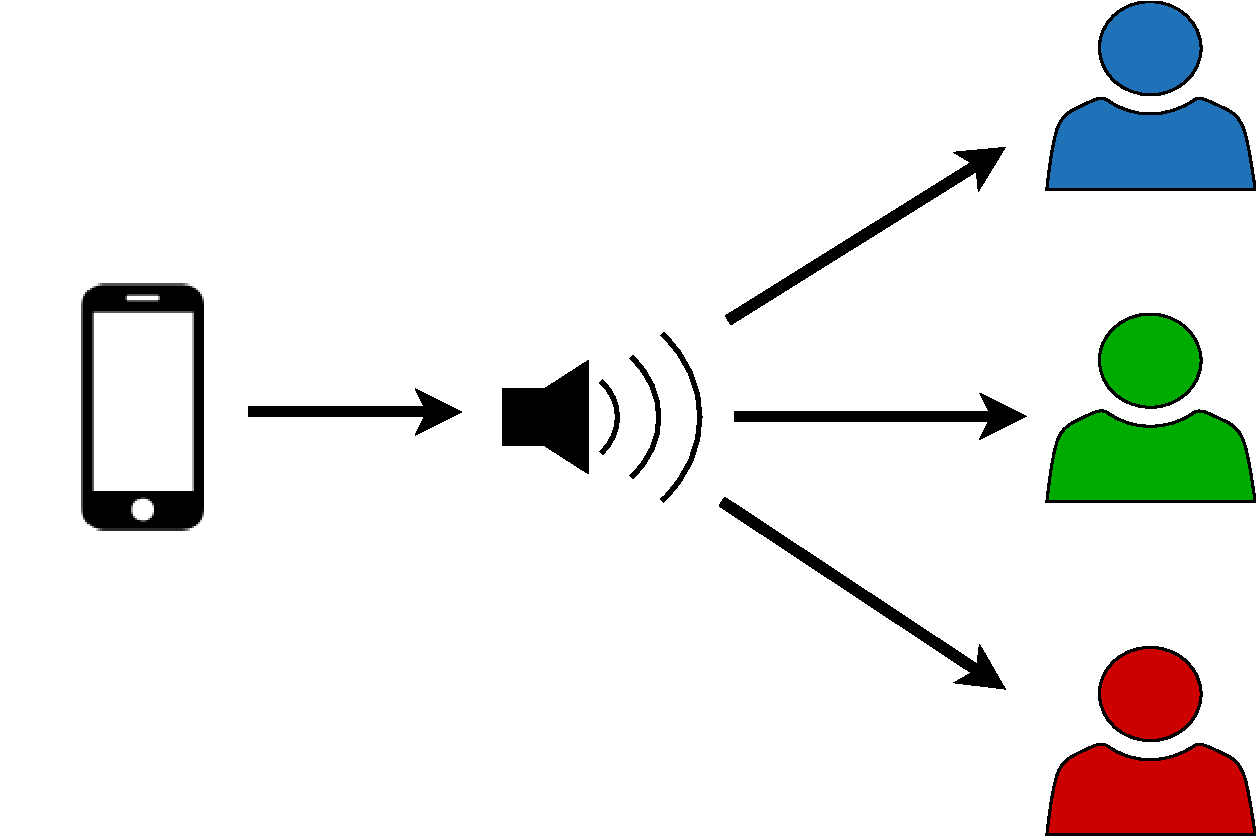
\includegraphics[width=0.45\textwidth]{speech_no_adapt}
		\label{fig:output_not_adapted}} 
	\hfill % no empty line here to avoid staring a new paragraph (figures will be vertically aligned)
	\subfigure
		[An illustration of a device's output, which is \emph{personalized} for each user.
		A different, customized spoken output (in blue, green, and red) is played to each user.]
		{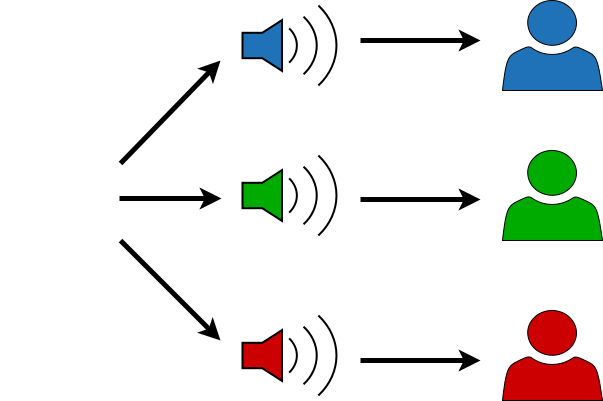
\includegraphics[width=0.45\textwidth]{speech_adapt}
		\label{fig:output_adapted}}
	\caption[Static vs.\ adaptive speech output]
		{Schematic comparison between an interaction with static spoken outputs (on the left) and an interaction with adaptive (i.e., personalized) spoken outputs (on the right).
		The system that adapts to the user makes the interaction tailored to the user's behavior.}
	\label{fig:static_vs_adaptive_speech_output}
\end{figure}

There are various motivations for speakers to change their behavior during spoken interactions.
This change can happen in different ways and on multiple levels \citep[][and see \cref{chap:phonetic_convergence} for more details]{Gallois2015CAT, Shepard2001CAT}, and the changes are mostly driven by external input of other interlocutors.
Many experiments have shown that vocal accommodation occurs in \ac{hhi} (and see \cref{chap:conv_analysis}), but only in recent years similar experiments were conducted and found similar effects in \ac{hci} as well (and see \cref{chap:shadowing_in_sung_music_and_human_computer_interaction,chap:speech_variations_in_hhci}).
However, while in \ac{hhi} the accommodation is, in its nature, mutual, in \ac{hci} only the human speaker could adjust voice characteristics.
This typically results in one-sided, weaker effects, as there is no counterpart to reinforce the process.
A major next step would be to add accommodation capabilities to \acp{sds} and make it mutual in \ac{hci}, too.
According to \citet{Weise2017towards}, integrating these capabilities into computer systems will enhance \ac{hci} and provide improved tools for studying accommodation also from the computers' side.
He also notes that accommodating dialogue systems could offer an additional layer of interaction, namely responding to user's behavior -- either by observing user's behavior and use it as additional information for some analyses or by actively making use of accommodation to encourage the user to speak in a specific way.
Though done in a more planned and direct way than in \ac{hhi}, this offers another level of dynamics from the system's side without changing the interaction's content.
\citet{Oviatt2004adaptive} discuss the advantages of systems that dynamically adapt their speech output to that of the user, and the challenges involved in developing and using these systems.

Dynamically changing the voice is a capability currently ascribed almost exclusively to humans and exist only sparsely and simplistically in computer-based systems.
As illustrated in \cref{fig:static_vs_adaptive_speech_output}, voice-activated devices always talk the same way, regardless of how the user speaks to them, the environment and setting in which the interaction takes place, the goal and role of the devices, etc.
This capability, which comes naturally to humans in social interactions, involves several steps of (partially unaware) decisions, which together form the overall effect of becoming behaviorally more or less similar to an interlocutor.
These include both situational and knowledge-related facets like how it is expected to behave in certain situations and which vocal changes fit those, as well as the physiological ability to apply these matches.
Humans can perform all these steps as one conduct.
For computers, however, these steps must be broken down, as they lack the common social background knowledge and the intuition as to how to match their voice to the situation.
Ultimately, \Acp{sds} with such personalized speech style may offer more natural and efficient interactions, as shown by \citet{Porzel2006entrainment}, and advance one more step away from the \emph{interface metaphor} \citep{Edlund2006twofaces} toward the \emph{human metaphor} \citep{Carlson2006humanlike}, to utilize new user approaches in spoken \ac{hci}.

A roadmap towards such systems is discussed in \cref{subsec:suggested roadmap} and terminology describing the different levels and ways to achieve accommodative vocal behavior in machines is introduced in \cref{subsec:accommodation_levels}.
Finally, examples of existing accommodative \acp{sds} are presented in \cref{subsec:systems_with_accommodation_capabilities}.

\subsection{Dialogue is hard}
\label{subsec:dialogue_is_hard}

As described in \cref{sec:linguistic_accommodation}, accommodation occurs naturally in \ac{hhi} as an integral part of dialogues.
The social conventions and unwritten rules of dialogue are implicitly learned by humans, who intuitively know how to apply them and when they can be altered.
This is an automatic process that is still too complex for integrating into computers.
Therefore, the way we interact with computers is often immensely different from communication with other human beings (\cref{subsec:verbal_interaction}), making it hard for computers to handle.
Another reason dialogue is hard is the infinitely many possible trajectories of each measured aspect.
It is always possible to create a dialogue that hasn't been produced before, even concerning a single aspect like chosen words, floor change, vocal properties, length, or any feature of any modality.
As if language understanding isn't a hard enough task for computers, the relations between all these aspects and their influence on one another make this task even more complex \citep{Gordon2018evaluating}.
The complexity of this task is long acknowledged and it was posed by \citet{Turing1950computing} as an \acs{ai}-complete problem.
Therefore, it is assumed that substantial, maybe human-like, intelligence is required to address its unexpected circumstance, and no specific algorithm or \ac{ml} method can solve it alone \citep[see further reasoning and examples in][pp.~54-57]{Shapiro1992encyclopedia}.
Notably, many aspects need to be explicitly split into separate steps and rules for the computer, although human process them as one concept (or at least don't consciously divide it into smaller sub-tasks).
One example of this is that humans don't strictly distinguish between task-oriented and chitchat dialogues (\cref{tab:sds_types}), whereas modeling approaches do.
Humans can also switch between the two, as they use both as part of one dynamic dialogue.
For example, people are good at having an off-topic small-talk at the beginning of a business meeting before switching, gradually or not, to the goal topic (cf.\ discussion about conversation structure and speaker role in \cref{subsec:conversation_intelligence}).
Furthermore, humans intuitively know how to behave based on the situational context, like when to take the floor, when to stop talking, when to barge in, etc., without the need for explicit signals from the other interlocutor.
Although there are approaches for teaching computers these dynamic changes \citep[e.g.,][]{Skantze2009incremental}, the gap is still substantial.

As a process that happens as part of a dialogue, accommodation involves some of these challenges (e.g., there may always occur pattern never seen before), but within a limited scope.
Moreover, accommodation entails the additional challenge of no \enquote{correct answer}, i.e., there is no measure of good or bad accommodation in a dialogue.
Humans might be able to point out if an interlocutor uses accommodation in an undoubtedly wrong way (for example, continuously perfectly imitating or demonstratively attempting to talk differently), but probably wouldn't notice how and whether their conversation partners accommodate to them.
This poses difficulties in both evaluation and learning, because it is not possible to put labels on accommodation measures without making numerous assumptions.
Therefore, the modeling approaches present in this work (\cref{chap:computational_model,chap:statistical_model}) concentrate on the \emph{behavior} of a speaker within a conversation rather than modeling how well accommodation was utilized.
The approach suggested in \cref{subsec:suggested roadmap} can be taken as a general scheme for any kind of mutual dynamics in \ac{hci}, which is here applied to vocal properties.

\subsection{Suggested roadmap}
\label{subsec:suggested roadmap}

The lack of accommodative speech in computer-based systems roots from what is more often than not natural and even automatic for humans, namely realizing how and how much to change their vocal behavior, the physiological means to express those differences, and the ability to combine the two into a coherent production in an interaction.
\Cref{fig:roadmap_adaptive_sds} shows an overview of a schematic roadmap to integrating adaptive capabilities into a \ac{sds}.
In addition to the standard functionality of the \ac{sds}, three main elements are required:
First, knowledge about the nature and properties of accommodative behaviors in humans is required.
This includes both empiric experimental data and integrable models.
% 1-2 sentence that at the moment there are many ways to measure accommodation and existing models are limited (reference? or at least point to terminology part)
Furthermore, the technical capability to control the speech output on demand is essential for introducing flexibility in the system's base voice.
This also includes a mechanism for accumulating phonetic evidence from the user's input relevant for the feature representations used for the accommodation process.
As these manipulations must be applied in real-time, re-training the \ac{tts} model to capture every change is not only insufficient but not practical as well.
This means that the manipulations are done on top of the existing \ac{tts} model, either by modifying the outputted waveform directly or by training a model that can consider specific changes in feature description (as done in \cref{subsec:speech_manipulation}).
To link between the modeled knowledge and the audio processing implementations, an additional component must be introduced in the system.
The role of this component is to feed the system's flexible voice parameters result from the models to express vocal changes, which are ultimately conveyed to the user.
This emphasizes the aforementioned notion of separating \emph{what} the system says (determined by the \ac{nlg} module) and \emph{how} to say it (to be determined by the \ac{tts} with the help of this additional component).

This work addresses each of those facets, each with its own challenges that require a profound work to investigate.
% (see the outline on pages \cpagerefrange{outline}{outline_end}).
%
\begin{figure}[t]
	\centering
	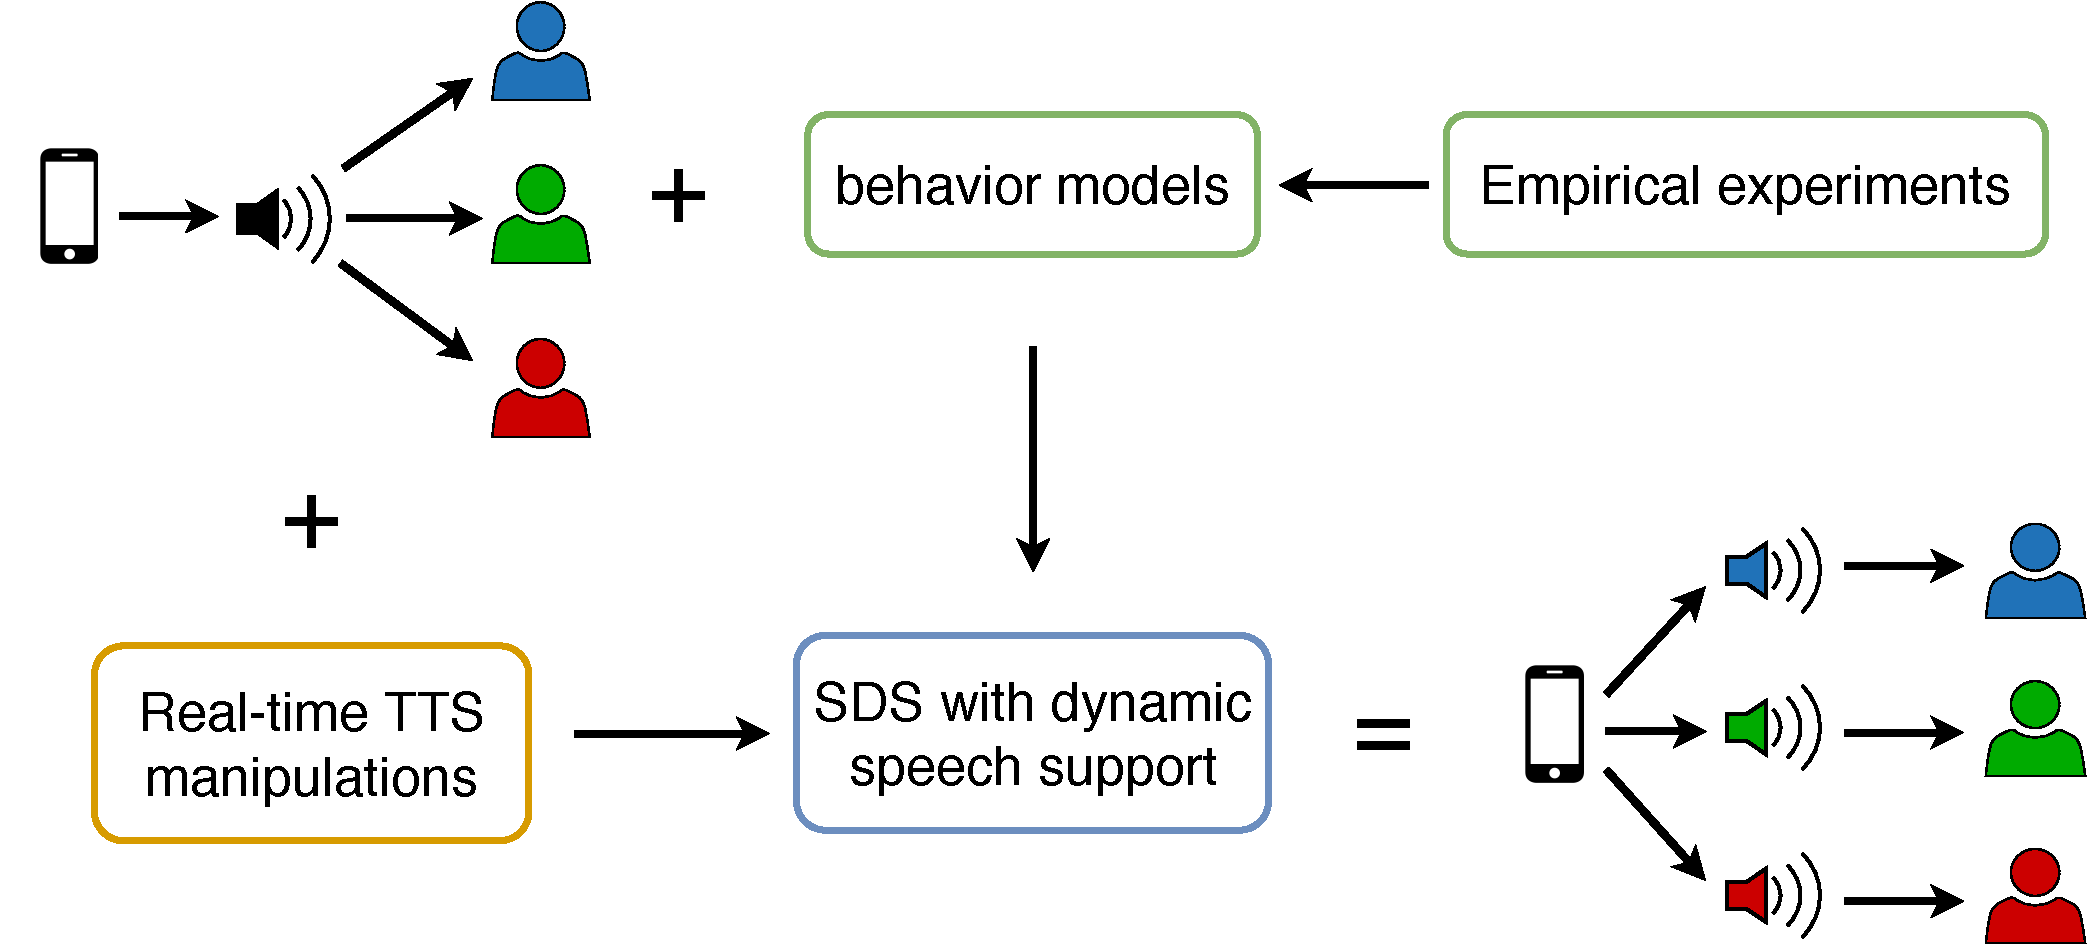
\includegraphics[width=\linewidth]{roadmap_adaptive_sds}
	\caption[Roadmap to phonetically adaptive \acl{sds}]
		{A suggested roadmap from static outputs (top left) to personalized outputs (bottom right) in \acp{sds} (and see \cref{fig:static_vs_adaptive_speech_output}).
		The green, orange, and blue blocks stand for the modeling, manipulation, and integration components described in the text, respectively.
		The \enquote*{+} signs represent direct addition to a static system and the arrows go from components required as a feed to others.}
	\label{fig:roadmap_adaptive_sds}
\end{figure}
%
For a \ac{sds} to accommodate its speech, it would not only need to support dynamic, on-demand changes of its \ac{tts} component's output, but would also need its \ac{asr} component to be able to identify and track specific features in the user's speech to update its representation of those features.
Completing the cycle, these representations can then be used as additional input for the \ac{tts} components to determine how those would influence the system's speech output.
This process is individual for each speaker and may occur over long periods or multiple interactions, depending on the desired degree and characteristics of accommodation.
Furthermore, this process may involve other components of the \ac{sds} as well.
For instance, the \ac{dm} might consider changes in the user's speech when making decisions, e.g., based on apparent mood and calmness.
The \ac{nlg} component could make alterations to its output to better fit the vocal changes of the system and the user's dynamic state, such as shortening sentences and omit additional information if phonetic indicators of hurry or urgency are detected in the speech input \citep{Edworthy2003acoustic}.

\subsection{Accommodation levels -- terminology}
\label{subsec:accommodation_levels}

In addition to all the above, another design choice for accommodative \acp{sds}, which is not explicitly required in human speech, concerns the overall \emph{level of accommodation} the system introduces.
This determines the fundamental behavior and form of variation in the system's speech, regardless of specific phonetic features, utterance contents, etc.
The variation levels (or properties) described below can potentially be combined in different ways to achieve the desired system behavior.
They are, at least to some extent, analogous to the aforementioned processes conducted by humans in social interactions, with the key difference that humans don't need to defined and think about them separately, if at all.
The utilization of these levels is demonstrated in the context of phonetic accommodation, which is one case of dynamic change of speech \citep{Weise2019individual, Schweitzer2016exemplar, Bevnuvs2014social}.
\Cref{chap:web-based_responsive_spoken_dialogue_system} further discusses and demonstrates the integration of such properties into a \ac{sds}.

Different terms are used in the literature to describe systems that can change their output.
This often leads to inconsistencies and mix-ups in terminology.
Definitions of five core properties of accommodative \ac{tts} that should, once accomplished, grant a more dynamic appearance, along with their suggested use and potential fusion with one another, are suggested below.
These terms seek to distinguish between the different capabilities that can be integrated into \acp{sds} and the way they relate to humans’ behaviors and each other.
%
\begin{description}
	\item[Adaptive] -- the vocal behavior evolves between and/or during interactions.\\
	This property refers to the system's use of any mean to \emph{dynamically} change its speech-related behavior, regardless of the source of influence or specific realizations.
%	Here, adapting means shifting the overall behaviors by updating a subset of the other properties.
	That means, for example, modifying the base behavior, extending the variability, or reflecting the system's changes earlier.
	This can happen between interactions or within a single, usually longer, interaction.
	The former could be more useful for \ac{cnc} systems or task-oriented \acp{sds} that are used by many users, while the latter is more suitable for social systems like chatbots and \acp{pa} (see \cref{sec:types_of_sdss}).
	Ultimately, this is a means for the system to improve its performance and accessibility based on previous interactions.
	However, for some applications, like a \ac{capt} system, for example, it would be better to \enquote{reset} their behavior between each use to offer a better experience.

	\item[Flexible] -- on-demand speech manipulation \emph{without retraining the voice}.\\
	This property refers to the technical capability to alter the system's speech output on request, which is achieved either via modifications in the voice's representation and parameters or by manipulating the outputted waveform directly using signal processing methods.
	Note that this does not entail the way this capability is used, and especially not that it is applied automatically.
	Moreover, as mentioned above, the technical capability to control the voice alone is not enough to create an accommodative behavior.
	This would also require additional data to be transferred to the \ac{tts} component to determine what manipulation to perform.
	To that end, the modeling steps can be built on top of this technical ground.
	It is important to note that this property compensates for the inherent ability in humans to control their voice at will, and therefore does not directly represent any specific element of humans' speech behavior like the other properties.
	
	\item[Responsive] -- changes are influenced by some \emph{external} speech input.\\
	A responsive system can, for instance, detect some target features in the user's speech input and, after comparing them to the system's representation of these features, guide the \ac{tts} on how to update them (typically, to make them more similar to the user's input).
	This requires a model that simulates these steps (as the one in \cref{chap:computational_model}).
	Yet this model would not have an independently defined behavior and it could only directly become more similar (or dissimilar) to the user in some fashion.
	Such models can be designed to imitate the user's immediate output from previous turns \citep[like in][]{Levitan2016implementing} or to gradually match it based on some parameters like sensitivity and interaction's history, as demonstrated in \citet{Raveh2017Interspeech}.
	This property represents the idea that humans change their speech (and behavior in general) when interacting with other people, which is a key aspect of the \ac{cat}.
	
	\item[Characterized (Profiled)] -- the system's voice has its own base behavior.\\
	Giving a \enquote{character} (or a \emph{profile}) to a voice means that it has a specified base behavior, which might include general properties of accommodation.
	This can also be seen as a \emph{role} the system plays in a conversation, e.g., if built based on a certain \ac{hhi} scenario \citep{Silber-Varod2018prosodic}.
	In that case, the system would try to stick to some pre-defined model, which contains the required information to fulfill said role.
	A system might also have several profiles to switch between based on the settings and goals of the interaction.
	In the context of accommodation, that would include, for example, the degree of accommodation, its timing, or how strongly the system will try to influence the user's speech.
	This property represents the fact that a human being has a certain -- however complex -- personality.
	More specifically, a vocal identity, which will be expressed in spoken interactions.
	This idea is the basis for the simulations presented in \cref{chap:statistical_model}, where each generative model can be seen as a core behavior.
	
	\item[Variable] -- variations on top of the base behavior are yielded.\\
	Some variations can be introduced based on the base profile.
	These are relatively minor differences that deviate from the voice's characteristics or enhance them in some way.
	From a system's point of view, the main purpose of such variations is to make the output style non-deterministic and therefore less repetitive and predictable.
	From the human point of view, this coincides with the difficulty to reproduce identical utterances in exactly the same way every time.
	Moreover, people, though having their individual personality, would speak differently based on various factors outside a conversation like their mood, the environmental conditions, time constraints, etc.
	This property comes, therefore, to grant some smaller-scale dynamics to the voice, in particular when its base behavior is deterministic.
	\Cref{chap:statistical_model} explains in details an approach to achieve such variational behaviors.
\end{description}
%

This work concentrates on facets concerning the properties \emph{responsive} (\cref{chap:computational_model}), \emph{characterized}, and \emph{variable} (\cref{chap:statistical_model}), which have been given little attention in \ac{sds} research.
Together, these properties result in a flexible, non-deterministic output derived from a defined core behavior, which might vary.
Added to the responsive output of a system, this creates a system that adapts to the user according to its own base behavior and probabilistic variations.

\subsection{Systems with accommodation capabilities}
\label{subsec:systems_with_accommodation_capabilities}

With the advancement of speech and \ac{nlp} technologies, the development of \acp{sds} has been accelerated in recent years.
These technologies are closing the gaps between computer and human speech quality and therefore help to investigate vocal accommodation in \ac{hci} with systems that can more closely simulate human performance.
Particularly, the overall quality and dynamic manipulation of modern \ac{tts} methods make it possible to change certain aspects in a system's voice (see \cref{subsec:speech_manipulation} for further details and examples).
\Acp{sds} with vocal accommodation capabilities typically focus on a few phonetic features at most, and sometimes only a single one.
Even though this does not provide a comprehensive coverage of all vocal changes that can be introduced in a conversation, the method of tracking and adapting the one feature can often be applied to others.
An overview of the development process of adaptive \acp{sds} and relevant methods is given by \citet{Levitan2020developing, Bernsen1998designing}.

\citet{Suzuki2003effects} introduce a system with pure prosodic vocal capabilities with no lexical content.
In an experiment, it communicated with the participants used hummed sounds with different \acf{f0}, intensity, and \enquote{speech} rate values.
The system was adapting to the participants to different degrees over the several interactions, after which the participants rated the system on different communication aspects, like cooperation and friendliness.
It was found that interaction series in which the system converged to the users with some degree of independence rather than cases where the system directly changed toward the user or completely mimicked the user's vocal behavior.
This is an important insight, since this is also not likely to happen in \ac{hhi}, as each speaker has a different general speaking style which varies differently if and when accommodating to an interlocutor (and see definitions in \cref{subsec:accommodation_levels}).
Another approach was taken by \citet{Acosta2011achieving}, whose system explicitly used mimicking for conveying emotions.
The assumption was that if participants use certain vocal characteristics to convey specific emotions, they would also perceive the same emotions from an interlocutor's speech with the same characteristics.
\citet{Lubold2015naturalness} investigated pitch accommodation in \ac{hci} with a system that supports different accommodation patterns.
One of these patterns was used while participants interacted with the system over multiple short tutoring sessions.
Ratings of perceived rapport showed that the method using pitch shifting of the system's pitch towards the user while keeping the original intonation was most successful.
Like before, these results are in line with the approach of converging with respect to some concrete features while retaining more general behavioral patterns.
Tackling vocal accommodation from a different direction, \citet{Ward2004automatic} developed a system that predicts the speech rate of phone operators based on their interlocutors' speech.
While the method was somewhat simplistic and was applied to monotonic conversations with predictable content, it nonetheless shows that some general tendencies can be found based on vocal behavior in a conversation.
As for implementation and integration, \citet{Levitan2016implementing} use a modular way for adding accommodation capabilities to a \ac{sds} while separating the technical methods from the modeling details.
This approach is similar to the one used in this work, with a major difference that here temporal aspects and non-linear methods were used to measure and analyze accommodation.
While the system in \citet{Levitan2016implementing} always directly converges towards the user at a defined rate, the modeling in this work aims to give the system an individual way to \emph{respond} to the user's behavior based on some core profile, as explained in \cref{subsec:accommodation_levels,fig:incr_gen_models}.

%\section{Evaluating spoken dialogue systems}
%\label{sec:evaluation_of_sdss}
%
%\todo[inline]{decide whether a section about evaluation is necessary}
%
%\ldots Therefore, evaluation of \acp{sds} depends on the purpose of the systems, which can be divided into two types, namely \textit{\aclp{tds}} and \textit{\aclp{ngs}}.
%
%\subsection{Task-driven Systems}
%\label{subsec:task-driven_systems}
%[doesn't really evaluate the \ac{sds}, but it's ability to predict what task should be performed]
%[typically part of a bigger system (which has a set of tasks it can perform (e.g., personal assistant))]
%
%\subsection{Non-goal Systems}
%\label{subsec:non-goal_systems}
%
%A \acf{ngs} is a \ac{sds} that does not necessarily aim to complete a specific task (unlike \acp{tds}).
%Its purpose is, then, more general and there might not even be a defined purpose for it.
%Chatbots (see \cref{subsec:chatbots}) are a good a example for a \ac{sds} that typically isn't used for accomplishing a practical task like getting information or operating a device.
%Instead, they are used as a long-term social companion (be it at home or as part of a mobile device) and even merely for entertainment.\todo{references for both examples}
%Since such systems don't help to achieve a defined goal, it is not possible to evaluate their performance based on how well (or whether at all) this goal task was carried out.
%There is a need therefore for another, more long-term and interaction-oriented method rather than a task-oriented method.
%On the one hand, from the \ac{hci} point of view, the advantage of such methods is that they evaluate the dialogue capabilities of the system and not merely it's ability to map speech patterns or keywords to a set pre-defined actions.
%On the other hand, however, the problem in such methods is that it is much harder to define metrics when the goal of the interaction is not completely defined.
%There are two approaches to solve this issue:
%The first is defining the 